% !TeX spellcheck = cs_CZ

\documentclass[11pt]{standalone}
\usepackage{siunitx}
\usepackage[usenames,x11names]{xcolor}
\usepackage{tikz}
\usepackage{pgfplots}
  \pgfplotsset{compat=newest}
  
\tikzstyle{level 1}=[level distance=5cm, sibling distance=1cm]
% Define styles for bags and leafs
\tikzstyle{bag} = [text width=14em, align=flush right]
\tikzstyle{end} = [text width=10em, align=flush left]
        
\begin{document}
  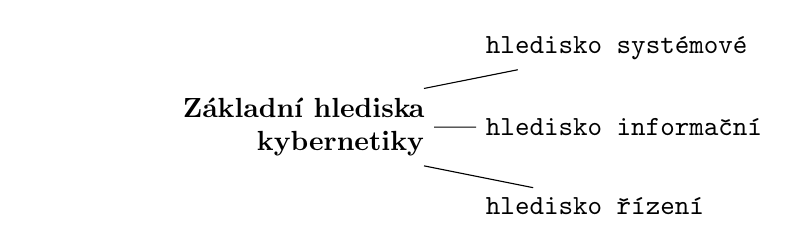
\begin{tikzpicture}[grow=right, sloped]
    \node[bag] {\textbf{Základní hlediska kybernetiky}}
        child {
            node[end] {\texttt{hledisko řízení}}
        }
        child {
            node[end] {\texttt{hledisko informační}}
        }
        child {
            node[end] {\texttt{hledisko systémové}}
        };
  \end{tikzpicture}
\end{document}
